\begin{comment}
\section{Event propagation}
HOPR uses a decentralized event propagation method (blockchain indexer) to allow information to be aggregated at many points in the network and shared with other nodes. 
This method prevents single point of failure vulnerabilities that service providers like infura or Alchemy could create. 
It also allows HOPR end users to use the HOPR network without needing any additional computational and bandwidth resources.  
\subsection*{HOPR decentralized trustless event propagation} 
HOPR uses Ethereum full nodes to fetch events and forward them to their HOPR instance which improves network latency.
HOPR then aggregates the events and store them chronologically:
\begin{itemize}
    \item $Open_i:=(c_{Id}, open, balance, balance_a)$
    \item $Close_i:=(c_{Id}, close)$
\end{itemize}
The nodes then publish the update independently to the DHT and allow HOPR end users to download it and verify the validity of the data.
\begin{figure}[H]
    \centering
    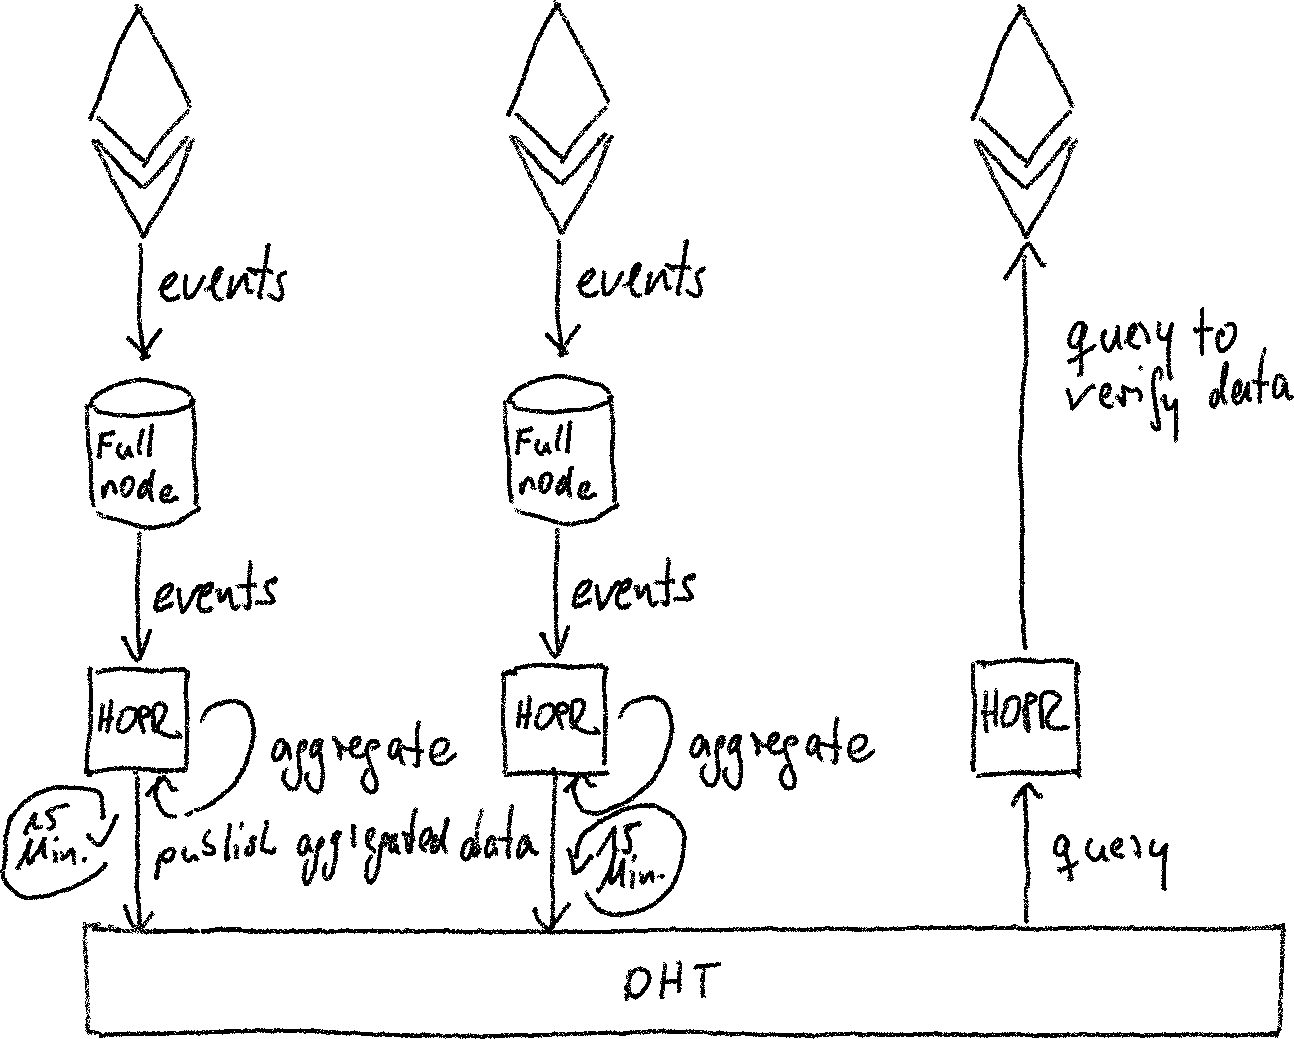
\includegraphics[width=7cm,height=7cm,keepaspectratio]{../yellowpaper/images/event_propagation.png}
    \caption{Event propagation}
    \label{fig:Event propagation}
\end{figure}
\hspace{-5mm}HOPR is a privacy preserving protocol that guarantees sender-receiver unlinkability while still providing high availability.
\\~In order to achieve the aforementioned properties, nodes use DHT to place information in the network and ask selected other nodes to replicate it and update that list every 5 minutes. Since the indexer retrieves on-chain information, there is no leakage about HOPR nodes' knowledge of the network. 
\\~Event logs are set to: $$log_i:=h( log_{i-1}|| Open) \quad or \quad log_i:=h( log_{i-1}|| Close )$$ where $log_0:=h(0)$.
\\~When a node receives $log_i$ from another node, the validity can be checked by recreating the hash and comparing the value with the on-chain value.

\end{comment}




